\documentclass[11pt]{standalone}
\usepackage{amssymb}
\usepackage{amsmath}
\usepackage[no-math]{fontspec}
\usepackage{unicode-math}
\usepackage{libertinus}
\usepackage{pgf,xcolor}
\usepackage{tikz}
\usetikzlibrary{arrows.meta, backgrounds, calc}
\usepackage{pgfplots}
\pgfplotsset{compat=newest}

\definecolor{my_darkgray}{HTML}{484949}
\definecolor{my_lightgray}{HTML}{F3F4F4}
\definecolor{my_darkblue}{HTML}{005A94}
\definecolor{my_lightblue}{HTML}{CCDEE9}
\definecolor{my_yellow}{HTML}{FFEC7F}
\definecolor{my_red}{HTML}{E60000}
\definecolor{my_orange}{HTML}{E87846}

\begin{document}
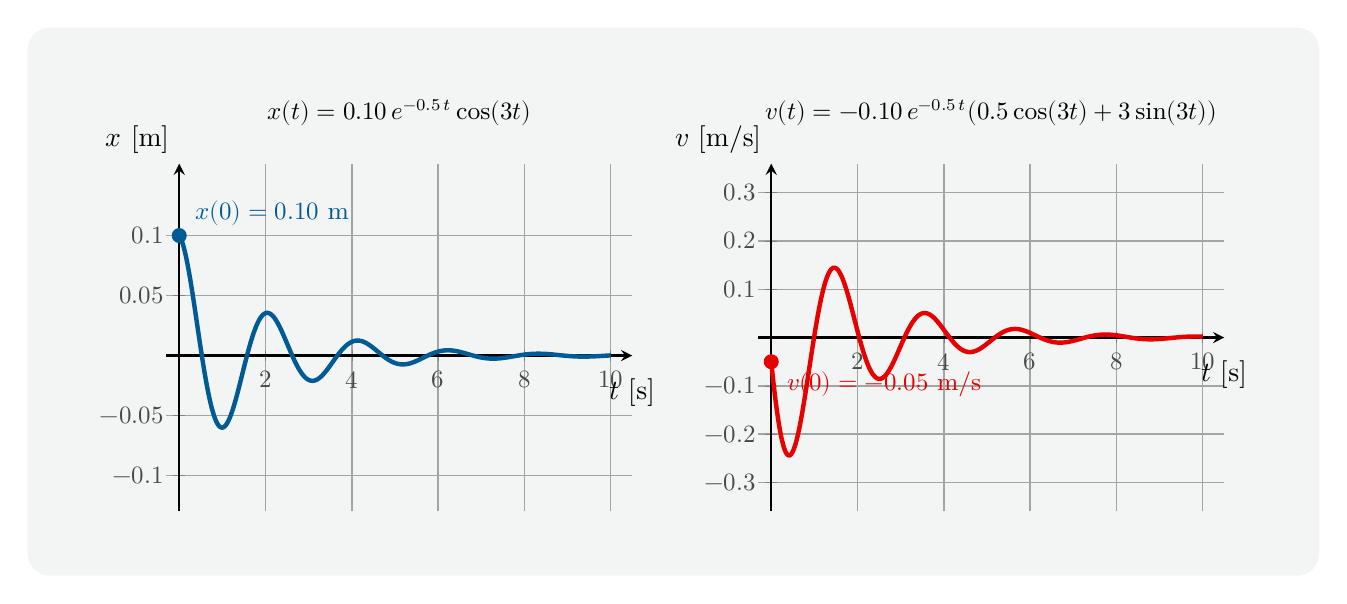
\begin{tikzpicture}[
    show background rectangle,
    background rectangle/.style={fill=my_lightgray, rounded corners=8pt},
    inner frame sep=0.8cm
]

% ── Left plot: x(t) = 0.10·e^(-0.5t)·cos(3t) ──────────────────────────────
\begin{axis}[
    name=left plot,
    axis lines = center,
    xlabel = {$t~[\text{s}]$},
    ylabel = {$x~[\text{m}]$},
    xlabel style = {at={(axis cs:10.5,0)}, anchor=north, yshift=-5pt},
    ylabel style = {anchor=south east},
    title = {$x(t) = 0.10\,e^{-0.5\,t}\cos(3t)$},
    title style = {font=\small, text=black, yshift=4pt},
    grid = both,
    grid style = {line width=0.3pt, draw=my_darkgray!30},
    major grid style = {line width=0.5pt, draw=my_darkgray!50},
    % axis equal omitted: x range 0..10 s vs y range ±0.10 m – very different scales
    axis line style = {thick},
    xmin = -0.3, xmax = 10.5,
    ymin = -0.13, ymax = 0.16,
    xtick = {0,2,4,6,8,10},
    ytick = {-0.10,-0.05,0,0.05,0.10},
    yticklabel style = {
        /pgf/number format/fixed,
        /pgf/number format/precision=2,
        font=\small,
        text=my_darkgray
    },
    xticklabel style = {font=\small, text=my_darkgray},
    width=7.5cm, height=6cm,
    clip=true,
]
\addplot[
    draw=my_darkblue,
    samples=600,
    ultra thick,
    domain=0:10
]{ 0.10 * exp(-0.5*x) * cos(deg(3*x)) };

% Mark the initial displacement x(0) = 0.10 m
\addplot[
    mark=*,
    mark size=2.5pt,
    only marks,
    draw=my_darkblue,
    fill=my_darkblue
] coordinates {(0, 0.10)};
\node[anchor=south west, font=\small, text=my_darkblue]
    at (axis cs:0.15, 0.10) {$x(0)=0.10~\text{m}$};
\end{axis}

% ── Right plot: v(t) = -0.10·e^(-0.5t)·(0.5·cos(3t) + 3·sin(3t)) ──────────
% Maximum amplitude of the oscillating factor: sqrt(0.5^2 + 3^2) ≈ 3.04,
% so |v|_max ≈ 0.10 × 3.04 ≈ 0.30 m/s near t = 0.
\begin{axis}[
    name=right plot,
    at={($(left plot.east)+(1.6cm,0)$)},
    anchor=west,
    axis lines = center,
    xlabel = {$t~[\text{s}]$},
    ylabel = {$v~[\text{m/s}]$},
    xlabel style = {at={(axis cs:10.5,0)}, anchor=north, yshift=-5pt},
    ylabel style = {anchor=south east},
    title = {$v(t) = -0.10\,e^{-0.5\,t}(0.5\cos(3t)+3\sin(3t))$},
    title style = {font=\small, text=black, yshift=4pt},
    grid = both,
    grid style = {line width=0.3pt, draw=my_darkgray!30},
    major grid style = {line width=0.5pt, draw=my_darkgray!50},
    % axis equal omitted: y range ±0.32 m/s vs x range 0..10 s
    axis line style = {thick},
    xmin = -0.3, xmax = 10.5,
    ymin = -0.36, ymax = 0.36,
    xtick = {0,2,4,6,8,10},
    ytick = {-0.30,-0.20,-0.10,0,0.10,0.20,0.30},
    yticklabel style = {
        /pgf/number format/fixed,
        /pgf/number format/precision=2,
        font=\small,
        text=my_darkgray
    },
    xticklabel style = {font=\small, text=my_darkgray},
    width=7.5cm, height=6cm,
    clip=true,
]
\addplot[
    draw=my_red,
    samples=600,
    ultra thick,
    domain=0:10
]{ -0.10 * exp(-0.5*x) * (0.5*cos(deg(3*x)) + 3*sin(deg(3*x))) };

% Mark the initial velocity v(0) = -0.05 m/s
\addplot[
    mark=*,
    mark size=2.5pt,
    only marks,
    draw=my_red,
    fill=my_red
] coordinates {(0, -0.05)};
\node[anchor=north west, font=\small, text=my_red]
    at (axis cs:0.15, -0.05) {$v(0)=-0.05~\text{m/s}$};
\end{axis}

\end{tikzpicture}
\end{document}
